\documentclass{beamer}
\usepackage{graphics}
\usepackage{epsfig}
\usepackage{algorithm}
\usepackage{verbatim}
\usepackage{listings}
\usepackage{framed}
\usepackage{flexiprogram}
\usepackage[UKenglish]{babel}
%\usepackage{psfrag}
\usepackage{hyperref}
\usepackage{pstricks}
\usepackage{pst-coil}
\usepackage{color}
\usepackage{epsfig}
\usepackage{tikz}
\usepackage{multirow}
%\usepackage{beamerthemesplit}
%\usepackage[pdflatex]{graphicx}
%\usepackage{helvet}
%\usepackage[T1]{fontenc}

\usefonttheme{serif}

\newtheorem{mydef}{Definition}
\newcommand{\ttf}[1]{{\tt #1}}
\newcommand{\tn}{\tabularnewline}
\newcommand{\rtarrow}{$\rightarrow$}
\newcommand{\mapp}{$\equiv$}
\newcommand{\bb}[1]{{\blue #1}}
\newcommand{\loc}{\ensuremath{l_0}}
\newcommand{\tnext}{\mbox{\tt next}}
\newcommand{\lt}{\mbox{\tt left}}
\newcommand{\rt}{\mbox{\tt right}}
\newcommand{\et}[1]{\emph{\tt #1}}
\newcommand{\isInterfering}{\mbox{isInterfering}}
\newcommand{\interf}[2]{\mbox{\sf interfere}(#1,\ #2)}
\newcommand{\flowdep}{\mbox{flow-dep}}
\newcommand{\antidep}{\mbox{anti-dep}}
\newcommand{\outputdep}{\mbox{output-dep}}
\newcommand{\rs}[1]{\mbox{read}(#1)}
\newcommand{\ws}[1]{\mbox{write}(#1)}
\newcommand{\rst}[2]{\mbox{read}(#1, #2)}
\newcommand{\wst}[2]{\mbox{write}(#1, #2)}
\newcommand{\set}{\mbox{set}}
%\noindent

\setcounter{tocdepth}{1}
\lstset{language=[ANSI]C}
\lstset{% general command to set parameter(s)
basicstyle=\footnotesize\tt, % print whole listing small
identifierstyle=, % nothing happens
commentstyle=\color{red}, % white comments
showstringspaces=false, % no special string spaces
lineskip=1pt,
captionpos=b,
frame=single,
breaklines=true
%\insertauthor[width={3cm},center,respectlinebreaks]
}
\lstset{classoffset=0,
morekeywords={},keywordstyle=\color{black},
classoffset=1,
classoffset=0}% restore default

\usetheme{Warsaw}
%\usecolortheme{dolphin}

\title{Heap Dependence Analysis for Sequential Programs}
\author[Presented by: Barnali Basak]{\large{\textbf{Barnali Basak}}
\vspace{0.2cm} 
\newline \small{Supervisors}
\vspace{0.1cm}
\newline \large{\textbf{Prof. Amey Karkare}}
\newline \small{\&}
\newline \large{\textbf{Prof. Sanjeev K. Aggarwal}}}
\institute{\textbf{Department of Computer Science and Engineering}
\newline \textbf{Indian Institute of Technology, Kanpur}}
\date{June 8, 2011}
%\begin{comment}
\begin{document}

\begin{frame}
\titlepage
\end{frame}

\AtBeginSection[]
{
\begin{frame}<beamer>
\frametitle{Outline}
\tableofcontents[currentsection]
\end{frame}
}

\section{Introduction}
\subsection{Introduction}
%\subsection{Motivation}
%\subsection{Related Work}
%\begin{comment}
\frame
{
	\frametitle{\subsecname}
	\uncover<1>{\textbf{Dependence Analysis : } produces execution order constraints between program statements. }
	\pause
	\begin{itemize}
	\item Data Dependences : Occurs due to data flow of program. 
	%\pause
	\begin{itemize}
	\item<2> Flow Dependence (Read after Write): \newline
	$\begin{array}{rcl}
	\tikz[baseline]{\node[fill=red!20,anchor=base]{x};} = a + b;\\
	y = \tikz[baseline]{\node[fill=blue!20,anchor=base]{x};} + z;
	\end{array}$ \\
%	\pause
	\item<3> Anti Dependence (Write after Read): \newline
	$\begin{array}{rcl}
	a = \tikz[baseline]{\node[fill=blue!20,anchor=base]{x};} + b;\\
	\tikz[baseline]{\node[fill=red!20,anchor=base]{x};} = y + z;
	\end{array}$ \\
%	\pause
	\item<4> Output Dependence (Write after Write): \newline
	$\begin{array}{rcl}
	\tikz[baseline]{\node[fill=red!20,anchor=base]{x};} = a + b;\\
	\tikz[baseline]{\node[fill=red!20,anchor=base]{x};} = y + z;
	\end{array}$ \\
%	\pause
	\end{itemize}
	\end{itemize}
%	\begin{program}{0}
%\UNL{0} 
\begin{center}
\tikz\node[fill=red!10,draw,circle] (n1){}; \small{Write access} %\newline
%\UNL{0} 
\tikz\node[fill=blue!10,draw,circle] (n2){}; \small{Read access}
\end{center}
%\end{program}
}
\frame
{
	\frametitle{\subsecname}
	\begin{center}
%	\begin{framed}
	$\begin{array}{lcl}
	for(i = 1; i <= n; i++) \{\\
	S1: x = a[i] + b;\\
	S2: a[i] = y + z;\\
	S3: a[i + 1] = x; \}
	\end{array}$ \\
	%\end{framed}
	\end{center}
	\begin{itemize}
	\item Loop Dependences : 	
	\begin{table}
	\centering
	\begin{tabular}{c c} %\hline %\hline
	\textbf{Iteration 1} & \textbf{Iteration 2} \\
	{$\begin{array}{lcl}
	S1: \tikz[baseline]{\node[fill=white!20,anchor=base]{x};} = \tikz[baseline]{\node[fill=blue!20,anchor=base]{a[1]};} + \tikz[baseline]{\node[fill=white!20,anchor=base]{b;};}\\
	S2: \tikz[baseline]{\node[fill=red!20,anchor=base]{a[1]};} = \tikz[baseline]{\node[fill=white!20,anchor=base]{y};} + \tikz[baseline]{\node[fill=white!20,anchor=base]{z;};}\\
	S3: \tikz[baseline]{\node[fill=white!20,anchor=base]{a[2]};} = \tikz[baseline]{\node[fill=white!20,anchor=base]{x;};} 
	\end{array}$}
	&
	{$\begin{array}{lcl}
	S1: \tikz[baseline]{\node[fill=white!20,anchor=base]{x};} = \tikz[baseline]{\node[fill=blue!20,anchor=base]{a[2]};} + \tikz[baseline]{\node[fill=white!20,anchor=base]{b;};}\\
	S2: \tikz[baseline]{\node[fill=red!20,anchor=base]{a[2]};} = \tikz[baseline]{\node[fill=white!20,anchor=base]{y};} + \tikz[baseline]{\node[fill=white!20,anchor=base]{z;};}\\
	S3: \tikz[baseline]{\node[fill=white!20,anchor=base]{a[3]};} = \tikz[baseline]{\node[fill=white!20,anchor=base]{x;};} 
	\end{array}$} \\

	\end{tabular}
	\end{table}
	\begin{itemize}
	\item Loop independent : $<S1, S2>$
	%\item<2> Loop carried : $<S3, S1>$ and $<S3, S2>$
	
	\end{itemize}
	
	\end{itemize}
	
}
\frame
{
	\frametitle{\subsecname}
	\begin{center}
%	\begin{framed}
	$\begin{array}{lcl}
	for(i = 1; i <= n; i++) \{\\
	S1: x = a[i] + b;\\
	S2: a[i] = y + z;\\
	S3: a[i + 1] = x; \}
	\end{array}$ \\
	%\end{framed}
	\end{center}
	\begin{itemize}
	\item Loop Dependences : 	
	\begin{table}
	\centering
	\begin{tabular}{c c} %\hline %\hline
	\textbf{Iteration 1} & \textbf{Iteration 2} \\
	{$\begin{array}{lcl}
	S1: \tikz[baseline]{\node[fill=white!20,anchor=base]{x};} = \tikz[baseline]{\node[fill=white!20,anchor=base]{a[1]};} + \tikz[baseline]{\node[fill=white!20,anchor=base]{b;};}\\
	S2: \tikz[baseline]{\node[fill=white!20,anchor=base]{a[1]};} = \tikz[baseline]{\node[fill=white!20,anchor=base]{y};} + \tikz[baseline]{\node[fill=white!20,anchor=base]{z;};}\\
	S3: \tikz[baseline]{\node[fill=red!20,anchor=base]{a[2]};} = \tikz[baseline]{\node[fill=white!20,anchor=base]{x;};}
	\end{array}$}
	&
	{$\begin{array}{lcl}
	S1: \tikz[baseline]{\node[fill=white!20,anchor=base]{x};} = \tikz[baseline]{\node[fill=blue!20,anchor=base]{a[2]};} + \tikz[baseline]{\node[fill=white!20,anchor=base]{b;};}\\
	S2: \tikz[baseline]{\node[fill=red!20,anchor=base]{a[2]};} = \tikz[baseline]{\node[fill=white!20,anchor=base]{y};} + \tikz[baseline]{\node[fill=white!20,anchor=base]{z;};}\\
	S3: \tikz[baseline]{\node[fill=white!20,anchor=base]{a[3]};} = \tikz[baseline]{\node[fill=white!20,anchor=base]{x;};}
	\end{array}$} \\

	\end{tabular}
	\end{table}
	\begin{itemize}
%	\item<1> Loop independent : $<S1, S2>$
	\item Loop carried : $<S3, S1>$ and $<S3, S2>$
	
	\end{itemize}
	
	\end{itemize}
	
}
\frame
{
	\frametitle{\subsecname}
	\textbf{Dependences arise due to :}
	\begin{itemize}
	\item scalars and pointers to stack allocated objects (stack-directed pointers) \\
%	\includegraphics[width=5cm]{test}\\
	\item pointers to heap heap allocated objects (heap-directed pointers)\\
	\end{itemize}
	\begin{figure}
	\begin{center}
%	\input{test}
	\scalebox{.95}{\begin{tabular}{ c  c }
	\input{fig_scalar}
	&
	\input{fig_heap} \\
%	(a) SDP & (b) HDP \\
	\end{tabular}}
%	\hrule
	\end{center}
	\end{figure}
%	\includegraphics[height=2cm]{img/proc1.jpg}
	
}
%\end{comment}

\frame
{
	\frametitle{\subsecname}

	\textbf{Difficulties in static analysis of heap :}
	
	\begin{itemize}
	\item Structure of heap is unknown.
	\item Size of heap structure is potentially unbounded.
	\item Lifetime of heap object is not limited by the scope that creates it.
	\item Presence of pointer induced aliasing, ex. \ttf{p\rtarrow{f}\rtarrow{f}} and \ttf{q\rtarrow{f}} access same heap object.
	\end{itemize}
}
\subsection{Motivation}
\frame
{
	\frametitle{\subsecname}
		
%	\begin{itemize}
%	\item \textbf{Fine grained parallelization} : in context of \textbf{\blue statements}
%	\item \textbf{Coarse grained parallelization} : in context of \textbf{\blue function calls}
%	\end{itemize}
	\begin{figure}
  \begin{center}
  
    \scalebox{.55}{\begin{tabular}[htbp]{ | c | c  |}
    \hline
    & \multirow{3}{*}{ \input{code_treeadd_colored_rw}} \\
%    & \\
      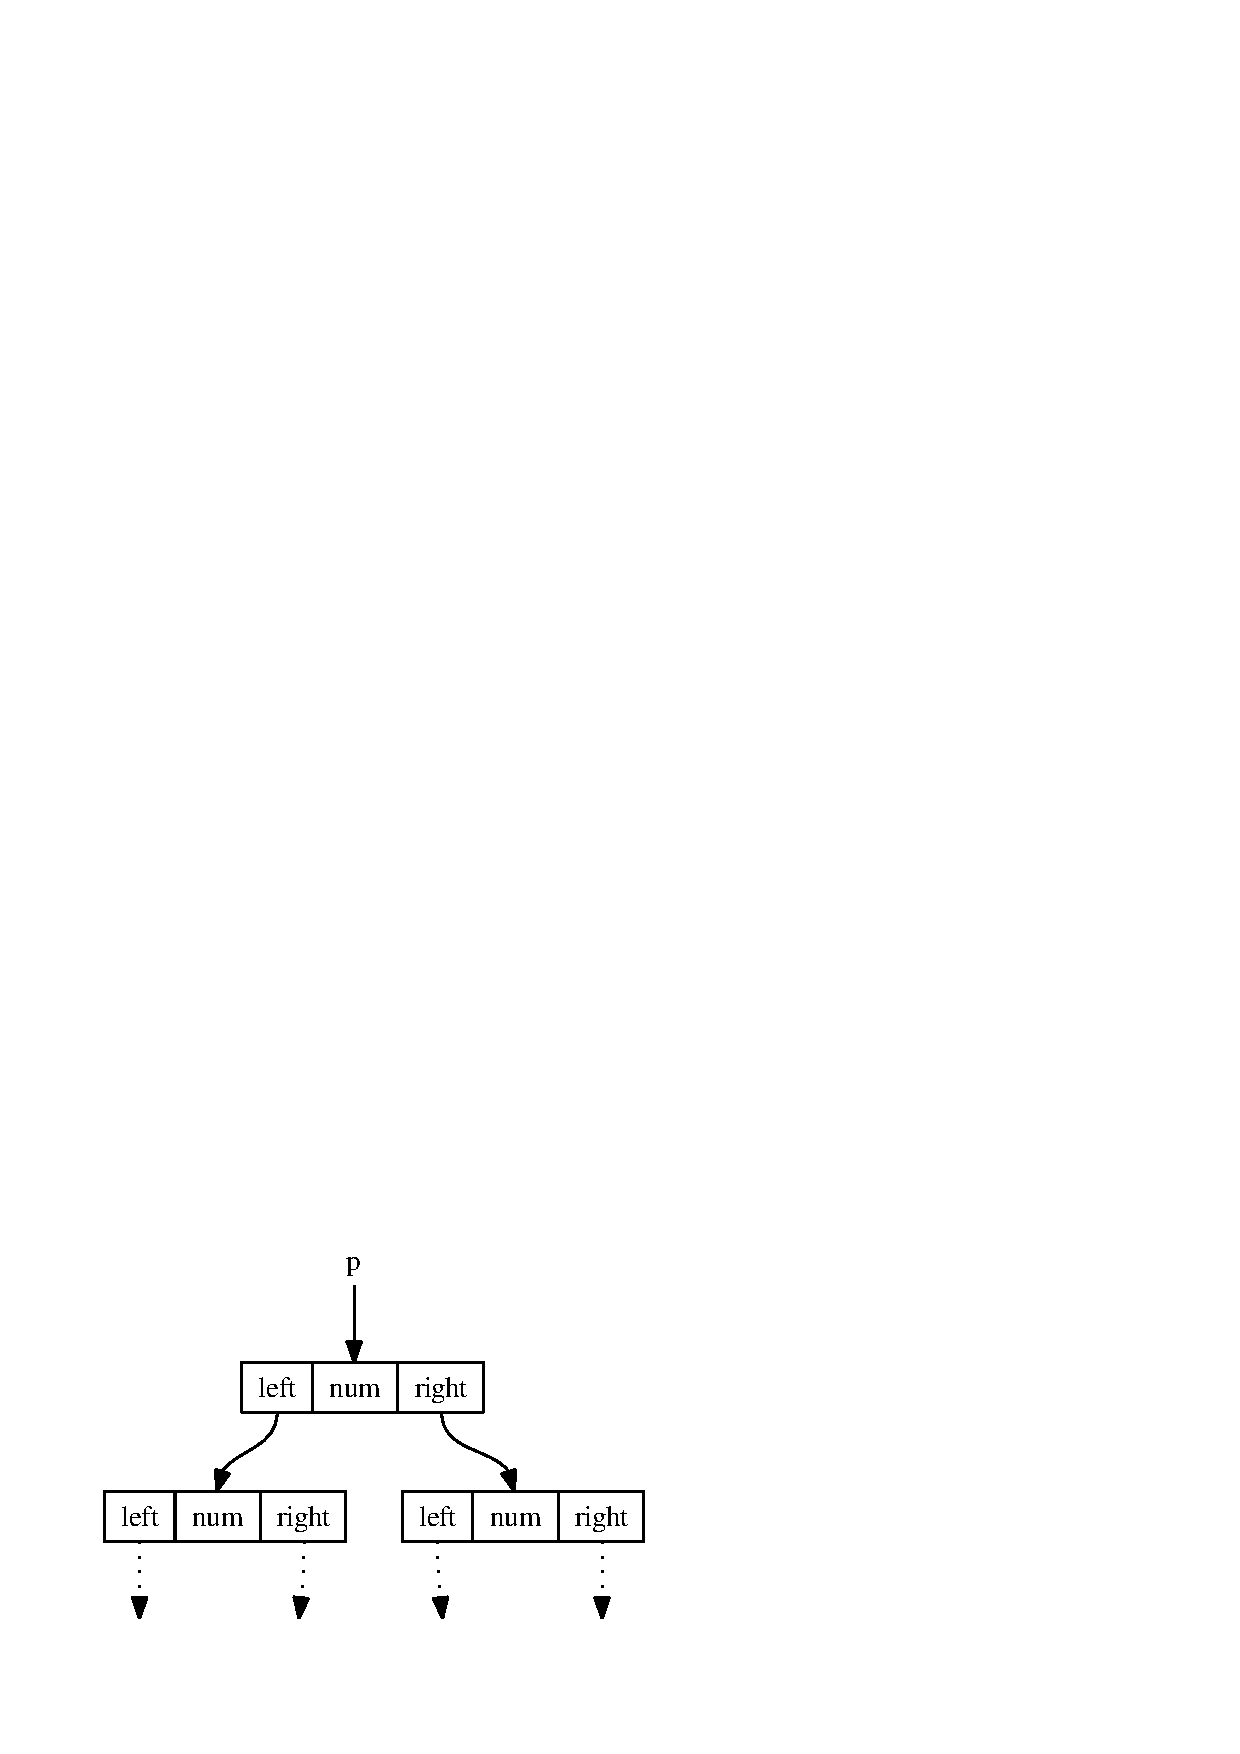
\includegraphics[scale=0.6]{tree_grph}
      & \\
 %     {\tt
\begin{program}{0}
%  \FL\ \ldots
  \UNL{0} void treeAdd(tree t) \{
  \UNL{1}  if(t == NULL)
  \UNL{2} return;
  \NL{1}     tl = t$\rightarrow$left;
  \NL{1}     treeAdd(tl);
  \NL{1}     tr = t$\rightarrow$right;
  \NL{1}     treeAddd(tr);
  \UNL{1}	t\rtarrow{num} = tl\rtarrow{num} + tr\rtarrow{num};
  \UNL{0} \}
\end{program}
} \\
     (a) Data structure & 
     (b Function traversing the data structure. \\
     \hline
    \end{tabular}}
  \end{center}
%  \caption{\label{fig:motiv1} Motivating example: function-call parallelization}
\end{figure}	
%\alert{mark the regions called by two functions}
}

\frame
{
	\frametitle{\subsecname}
%	\begin{itemize}
%	\item \textbf{Coarse grained parallelization} : in context of \textbf{\blue loops}
%	\end{itemize}	
	\begin{figure}
  \begin{center}
  
    \scalebox{.55}{\begin{tabular}{| c | c |}
    \hline
      \includegraphics[scale=0.5]{grph4} %\cline{1-1}
      &
      \input{fig_motiv_colored} \\
      \includegraphics[scale=0.5]{grph_motiv} & \\
%      (a) & (b) \\
     (a) Nodes read and written by code & 
     (b) Loop traversing the data structure. \\
     \hline
    \end{tabular}}
  \end{center}
%  \hrule
%  \caption{\label{fig:motiv} Motivating example: loop parallelization}
%\hrule
\end{figure}
}
\subsection{Objective}
\frame
{
	\frametitle{\subsecname}
	\begin{itemize}
	\item Intraprocedural analysis 
	\begin{itemize}
	\item works on each procedure separately, does not cross process boundary
	\item finds out both fine grained and coarse grained parallelism
	\end{itemize}
	\pause
	\item Loop sensitive analysis 
	\begin{itemize}
	\item targets loop sensitive processes
	\item efficiently extracts loop level parallelism
	\end{itemize}
	\pause
	\item Interprocedural analysis 
	\begin{itemize}
	\item works on whole program, crosses process boundary
	\item handles function calls more efficiently
	\end{itemize}
	\end{itemize}
}
\subsection{Programming Model}
\begin{comment}
\frame
{
	\frametitle{\subsecname}
	\begin{itemize}
	\item Heap allocating statements : {\tt p = malloc()}

	\item Pointers assigning statements :
	\begin{itemize}
	\item {\tt p = q} 
	\item {\tt p = q$\rightarrow$f} 
	\item {\tt p = NULL}
	\end{itemize}

	\item Link defining/ structure updating statements :
	\begin{itemize}
	\item {\tt p$\rightarrow$f = NULL} 
	\item {\tt p$\rightarrow$f = q}
	\end{itemize}

	\item Heap reading/ writing statements : 
	\begin{itemize}
	\item {\tt $\cdots$ = p$\rightarrow$data} 
	\item {\tt p$\rightarrow$data = $\cdots$} 
	\end{itemize}
	\end{itemize}	
}
\end{comment}
\frame
{
	\frametitle{\subsecname}
	
\begin{figure}
  \begin{center}
  
    \scalebox{.7}{\begin{tabular}{ | c | c | c | c |}
   \hline
   & Before execution & Statement & After execution \\
   \hline
    Allocations & \input{fig_ptrassgn_3_after} & \ttf{p = malloc()} & \input{fig_malloc}\\
    \hline
    \multirow{3}{*}{Pointer Assignments} & \input{fig_ptrassgn_1} & \ttf{p = q} & \input{fig_ptrassgn_1_after} \\
    \cline{2-4}
    & \input{fig_ptrassgn_2} & \ttf{p = q\rtarrow{f}} & \input{fig_ptrassgn_2_after} \\
    \cline{2-4}
    & \input{fig_malloc} & \ttf{p = NULL} & \input{fig_ptrassgn_3_after} \\
     \hline
     \multirow{2}{*}{Structure updates} & \input{ptr_strup_1} & \ttf{p\rtarrow{f} = NULL} & \input{ptr_strup_1_after} \\
     \cline{2-4}
     & \input{ptr_strup_2} & \ttf{p\rtarrow{f} = q} & \begin{pspicture}(0,3)(3,5.2)
\psset{linecolor=blue}
\pscircle(1.3,4.5){.3}
\pscircle(2.7,4.5){.3}
\pscircle(2,3.5){.3}
\psset{linecolor=black}
\psline[linewidth=1pt,linearc=.5]{->}(0.4,4.5)(1,4.5)
\psline[linewidth=1pt,linearc=.5]{->}(1.1,3.5)(1.7,3.5)
\psline[linewidth=1pt,linearc=.5]{->}(1.3,4.2)(2,3.8)
\rput(0.2,4.5){\psframebox*{\scalebox{1}{\ttf{p}}}}
\rput(1.6,4){\psframebox*{\scalebox{1}{\ttf{f}}}}
\rput(0.9,3.5){\psframebox*{\scalebox{1}{\ttf{q}}}}
\end{pspicture}
 \\
     \hline
    \end{tabular}}
  \end{center}
\end{figure}
}
\frame
{
	\frametitle{\subsecname}
	
\begin{figure}
  \begin{center}
  
    \scalebox{.7}{\begin{tabular}{ | c | c | c | c |}
     \hline
   & Before execution & Statement & After execution \\
   \hline
   \multirow{2}{*}{Heap reading/writing} & \input{fig_before_rdwr} & \ttf{a = p\rtarrow{data}} & \input{fig_heap_read} \\
   \cline{2-4}
   & \input{fig_before_rdwr} & \ttf{p\rtarrow{data} = a} & \input{fig_heap_write} \\
   \hline
   \end{tabular}}
   \end{center}
   \end{figure}
%   \begin{center}
   \centering{\blue Statements are normalized}
   \begin{figure}
  \begin{center}
  \scalebox{.7}{\begin{tabular}{  c  c }
  {$\begin{array}{lcl}
	\ttf{x = p\rightarrow{f}\rightarrow{data}}
	\end{array}$} 
	&
	{$\begin{array}{lcl}
	\ttf{q = p\rightarrow{f}} \\
	\ttf{x = q\rightarrow{data}} 
	\end{array}$} 
    \end{tabular}}
   \end{center}
   \end{figure}
}

\section{Intra-Procedural Dependence Analysis}

\subsection{Workflow}
\frame
{
	\frametitle{\subsecname}  
	Steps of intraprocedural analysis :
	\newline
	\begin{itemize}
	\item \textbf{Preprocessing - Initialization and Annotation}
	\end{itemize}
	\begin{itemize}
	\item \textbf{Computation of Read and Write sets of abstract access paths}
	\end{itemize}
	\begin{itemize}
	\item \textbf{Detection of dependences}
	\end{itemize}	
}
\subsection{Preprocessing}
\frame
{
	\frametitle{\subsecname}
	\begin{itemize}
	\item<1> Initialize global pointer variables and pointer parameters to symbolic locations.
	\item<2> Annotate statements with tagging directive, consisting of four attributes
	\begin{itemize}
	\item {Used pointer set} 
	\item {Defined pointer set}
	\item {Access field} 
	\item {Access type}
	\end{itemize}
	\end{itemize}
	
}

\frame
{
	\frametitle{\subsecname}
%	\begin{itemize}
%	\begin{itemize}
	\begin{figure}
	\begin{center}
	\scalebox{0.8}{\begin{tabular}{| c | c | c | c | c |}
	\hline
	Stmt & Used ptr & Def ptr & Acc field & Acc type\\
	\hline
	\ttf{p = q} & \ttf{\{q\}} & \ttf{\{p\}} & \ttf{Null} & alias \\
	\ttf{p = q\rtarrow{next}} & \ttf{\{q\}} & \ttf{\{p\}} & \ttf{next} & link trav\\
	\ttf{$\cdots$ = p\rtarrow{data}} & \ttf{\{p\}} & \ttf{\{\}} & \ttf{Null} & read heap \\
	\ttf{p\rtarrow{data} = $\cdots$} & \ttf{\{p\}} & \ttf{\{\}} &\ttf{Null} & write heap \\
	\ttf{fun(p, q)} & \ttf{\{p, q\}} & \ttf{\{\}} & \ttf{Null} & func call \\
	\hline
	\end{tabular}}
	\end{center}
	\end{figure}
	
%	\end{itemize}
%	\end{itemize}
}
\subsection{Computation of Read and Write Sets}
%\subsection{Access Path Abstraction}
\frame
{
	\frametitle{\subsecname}                                                  
	\begin{itemize}
	\item \textbf{Access Path :} symbolic heap location $\ttf{l_0}$ or location followed by pointer fields like $\ttf{l_0}\rightarrow\ttf{f_1}\rightarrow\cdots\rightarrow\ttf{f_k}$
	\end{itemize}
	\begin{figure}
	\begin{center}
	\scalebox{.6}{
	\input{fig_access_path} }
	\end{center}
	\end{figure}
	\pause
	\begin{itemize}
	\item \textbf{Abstraction Scheme :}  
	\begin{itemize}
	\item Length of access path is limited to length \ttf{k}. 
	\item Summary field `*' abstracts fields dereferenced beyond length \ttf{k}. ({\blue Here k = 1})
	\end{itemize}
	\end{itemize}
	\begin{figure}
	\begin{center}
	\scalebox{.6}{
	\input{fig_abstract_path} }
	\end{center}
	\end{figure}
	
	
}
\frame
{
	\frametitle{\subsecname}
	\textbf{State Analysis :} %Follows flow sensitive data flow analysis~\cite{Kam76globaldata, Muchnick97, Cooper02, Khedker09} etc.
	\begin{mydef}{
The state of heap directed pointer variable {\tt x} at a program point {\tt u} is the set symbolic memory locations such that some paths from the {\tt Entry} point to {\tt u} result in the access of symbolic locations by the variable \ttf{x}. }
\end{mydef}
\pause
\begin{figure}
	\begin{center}
	\scalebox{.6}{
	\input{fig_state_flow} }
	\end{center}
	\end{figure}
}
\frame
{
	\frametitle{\subsecname}
	\textbf{State Analysis :}	
	\begin{itemize}
	\item control flow sensitive forward-flow analysis
%	\item works on basic block instead of statement
	\end{itemize}
	\begin{figure}
%\hrule
\begin{center}
\begin{framed}
\scalebox{.6}{
\input{state_anal} }
%\small{Algorithm for state analysis}
\end{framed}
\small{Top level algorithm of state analysis}
\end{center}
%\small{Algorithm for state analysis}
\end{figure}
	
}

\frame
{
	\frametitle{\subsecname}
\begin{figure}[t]
  \begin{center}
  
    \scalebox{.6}{\begin{tabular}{| c | c |}
   \hline
     \input{fig_transfer_func_colored}
      &
      \input{fig_stmt_trans} \\ %\cline{2-2} 
      \hline
      & \\
     $\ttf{f_{B_3}(In[B_3])=g_{S_k}(\cdots(g_{S_1}(In[B_3])))}$ & $\ttf{g_{S_i}(In[S_i])=(In[S_i]-Kill[S_i])\bigcup{Gen[S_i]}}$ \\
     & \\
      %\hline
      \hline
    \end{tabular}}
  \end{center}
\end{figure}	
}
\frame
{
	\frametitle{\subsecname}
	\textbf{Gen and kill sets of statements :}
	\begin{figure}
	\centering
	\scalebox{.65}{\begin{tabular}{|l|c|c|} 
	\hline %\hline
	Statement & Gen set & Kill set \\
\hline %\hline
{\tt p = q} & {\tt \{<p,m> | <q,m>$\in$In[S]\}} & {\tt \{<p,l> | <p,l>$\in$In[S]\}} \\
{\tt p = q\rtarrow{next}} & {\tt \{<p,m\rtarrow next> | <q,m>$\in$In[S]\}} & {\tt \{<p,l> | <q,l>$\in$In[S]\}} \\
{\tt $\cdots$ = p\rtarrow{data}} & \{\} & \{\} \\
{\tt p$\rightarrow$data = $\cdots$} & \{\} & \{\} \\
{\tt fun(p,q)} & \{\} & \{\} \\
\hline
	\end{tabular}}
%	\caption{Heart beat and blood pressure using different monitoring methods}
%	\label{tbl:kramer}
	\end{figure}
\pause
	\textbf{Read/Write set of treeAdd function :}
	\begin{figure}
  	\begin{center} 
    \scalebox{.6}{\begin{tabular}{ | c | c | }
  	\hline
      \input{code_treeadd_colored_rw}
      &
      \scalebox{.8}{\begin{tabular}{c}
      \scalebox{.9}{\begin{tabular}{ | l | c | }
       \hline
        \multicolumn{2}{|c|}{Initialization : $\ttf{\{<t,l_0>\}}$ }\\
        \hline %\hline 
       Stmt & State \\
       \hline
       S1 & $\ttf{\{<t,l_0>,<tl,l_0\rightarrow{left}>\}}$\\
       S3 & $\ttf{\{<t,l_0>,<tl,l_0\rightarrow{right}>\}}$\\
       \hline
       
       \end{tabular}} \\
       Shows state \\
       \\ 
       \\
     \scalebox{.9}{\begin{tabular}{ | l | c | c | }
     \hline
     Stmt & Read set & Write set \\
     \hline
     S2 & \ttf{<tl,$l_0\rightarrow${left}>,} & \ttf{<tl,$l_0\rightarrow${left}>,} \\
      & \ttf{<tl,$l_0\rightarrow${left}$\rightarrow${*}>\}} & \ttf{<tl,$l_0\rightarrow${left}$\rightarrow${*}>\}} \\
     S4 & \ttf{<tr,$l_0\rightarrow${right}>,} & \ttf{<tr,$l_0\rightarrow${right}>,} \\
      & \ttf{<tr,$l_0\rightarrow${right}$\rightarrow${*}>\}} & \ttf{<tr,$l_0\rightarrow${right}$\rightarrow${*}>\}} \\
      \hline
     \end{tabular}} \\
     Shows read/write sets \\
     \end{tabular}} \\
     \hline
    \end{tabular}}
  \end{center}
\end{figure}
}

%\subsection{Read and Write Set Computation}
\begin{comment}
\frame
{
	\frametitle{\subsecname}
	\textbf{Example showing state analysis}
	\begin{figure}
  \begin{center}
  
    \scalebox{.65}{\begin{tabular}{| c | c |}
  	 \hline
      \input{code_treeadd_colored}
      &
      
       \scalebox{.85}{\begin{tabular}{ | l | c | }
       \hline
        \multicolumn{2}{|c|}{Initialization : $\ttf{\{<t,l_0>\}}$ }\\
        \hline %\hline 
       Stmt & State \\
       \hline
       S1 & $\ttf{\{<t,l_0>,<tl,l_0\rightarrow{left}>\}}$\\
       S3 & $\ttf{\{<t,l_0>,<tl,l_0\rightarrow{right}>\}}$\\
       \hline
       \end{tabular}} \\
       \hline
    \end{tabular}}
  \end{center}
\end{figure}		
}
\end{comment}

\subsection{Dependence Detection}
\frame
{
	\frametitle{\subsecname}
	\begin{itemize}
	\item Two access paths \ttf{p.$\alpha'$} and \ttf{q.$\beta'$} interfere if 
	\[\isInterfering(p, \alpha, q, \beta) = True\]	
	 $\alpha$ and $\beta$ are prefixes of $\alpha'$ and $\beta'$.
	 \pause
	\item Statements \ttf{S} and \ttf{T} are dependent on each other if 
%	$\begin{array}{rcl}
\[\interf{\set_1}{\set_2} \equiv \isInterfering(p, \alpha, q,
\beta)\]
p.$\alpha\in{set_1}$, q.$\beta\in{set_2}$
\pause
\begin{framed}
\[\flowdep(S, T) \equiv \interf{\ws{S}}{\rs{T}} \]
\[\antidep(S, T) \equiv \interf{\rs{S}}{\ws{T}} \]
\[\outputdep(S, T) \equiv \interf{\ws{S}}{\ws{T}} \]
\end{framed}
%\end{array}$ \\
%\end{itemize}
\end{itemize}
}

\frame
{
	\frametitle{\subsecname}
	\textbf{Detecting dependence between function calls :}
	\begin{figure}
  \begin{center}
  
    \scalebox{.65}{\begin{tabular}{| c | c |}
  	 \hline
      \input{code_treeadd_colored_rw}
      &
      
       \scalebox{.7}{\begin{tabular}{ | c | c | c | }
       \hline
        \multicolumn{3}{|c|}{Dependence Detection}\\
        \hline %\hline 
       Query & Predicate & Dependence\\
       \hline
       {flow-dep(S2,S4)} & \multirow{4}{*}{{isInterfering(t,left,t,right)}} & \multirow{4}{*}{No}\\
	   {anti-dep(S2,S4)} & & \\
	   {output-dep(S2,S4)} & & \\      
       \hline
       \end{tabular}} \\
       & Detects dependence \\
       \hline
    \end{tabular}}
  \end{center}
\end{figure}		
}
\frame
{
	\frametitle{\subsecname}
	\textbf{Detecting dependence of loop :}
	\begin{figure}
  \begin{center}
  
    \scalebox{.65}{\begin{tabular}{| c | c |}
  	 \hline
      \input{fig_motiv_colored}
      &
      \scalebox{.85}{\begin{tabular}{c}
        \scalebox{.9}{\begin{tabular}{ | l | c | c | }
     \hline
     Stmt & Read set & Write set \\
     \hline
     S3 & \ttf{<q,$l_0\rightarrow${next}>,} & \{\} \\
      & \ttf{<q,$l_0\rightarrow${next}$\rightarrow${*}>\}} & \\
     S5 & \{\} & \ttf{<r,$l_0\rightarrow${next}$\rightarrow${*}>,} \\
      \hline
     \end{tabular}} \\
     Shows read/write sets \\
     \\
     \\
     \scalebox{.9}{\begin{tabular}{ | c | c | c | }
       \hline
        \multicolumn{3}{|c|}{Dependence Detection}\\
        \hline %\hline 
       Query & Predicate & Dependence\\
       \hline
       {flow-dep(S3,S5)} & \multirow{4}{*}{{isInterfering(p,next,p,next)}} & {No}\\
	   {\red anti-dep(S3,S5)} & & {\red Yes}\\
	   {output-dep(S3,S5)} & & No\\      
       \hline
      \end{tabular}} \\
       Detects dependence \\
     \end{tabular}} \\
     \hline
    \end{tabular}}
  \end{center}
\end{figure}
}
\subsection{Shortcomings}
\frame
{
	\frametitle{\subsecname}
	\begin{itemize}
	\item Does not perform well in presence of loops
	\end{itemize}
	\begin{itemize}
	\item Considers worst case summary of called functions
	\end{itemize}
	\begin{itemize}
	\item Imprecise for both loop level and function level parallelism
	\end{itemize}
}
\section{Loop Sensitive Dependence Analysis}
\subsection{Workflow}
\frame
{
	\frametitle{\subsecname}
	Steps of loop sensitive analysis :
	\newline
	\begin{itemize}
	\item \textbf{Identification of navigator variable and navigator expression}
	\end{itemize}
	\begin{itemize}
	\item \textbf{Computation of Read and Write sets of complete access paths}
	\end{itemize}
	\begin{itemize}
	\item \textbf{Detection of dependences (both loop independent and loop carried)}
	\end{itemize}
	
}
\subsection{Identifying Navigator}
\frame
{
	\frametitle{\subsecname}
	Navigator of loop consists of :
	\begin{itemize}
	\item navigator variable : pointer variable used to traverse loop
	\item navigator expression : sequence of pointer field references to navigate loop
	\end{itemize}
	
	\begin{figure}
	\begin{center}
	 \scalebox{.6}{\begin{tabular}{| c | c | }
	 \hline
      \input{fig_code_no_dep} & \input{fig_code_dep} \\
      navigator variable : {\blue \ttf{p}} & navigator variable : {\blue \ttf{p}} \\
      navigator expression : {\blue \ttf{next\rtarrow{next}}} & navigator expression : {\blue \ttf{next}} \\
      \hline
      \end{tabular}}
  \end{center}
\end{figure}
}
\subsection{Detecting Dependence}
\frame{
	\frametitle{\subsecname}
	\textbf{Loop Independent Dependence :}
	\begin{description}
	\item<1>[Observation 1:] If shape is Tree
	\begin{itemize}
	\item \ttf{p\rtarrow{f}\rtarrow{f}} and \ttf{p\rtarrow{f}\rtarrow{g}} do not access common node
	\item \ttf{p\rtarrow{f}\rtarrow{f}} and \ttf{p\rtarrow{f}\rtarrow{f}} always access common node
	\end{itemize}
	\item<2>[Observation 2:] If shape is DAG
	\begin{itemize}
	\item \ttf{p\rtarrow{f}} and \ttf{p\rtarrow{f}\rtarrow{g}} do not access common node as former path is proper subpath of later path
	\item \ttf{p\rtarrow{f}\rtarrow{f}} and \ttf{p\rtarrow{f}\rtarrow{g}} can potentially access common node
	\end{itemize}
	\end{description}
}

\frame{
	\frametitle{\subsecname}
	\begin{figure}
	\begin{center}
	 \scalebox{.6}{\begin{tabular}{| c | c |} 
	 \hline
      \input{fig_code_no_colored} & \input{fig_code_dep_colored} \\
       navigator variable : {\blue \ttf{p}} & navigator variable : {\blue \ttf{p}} \\
     navigator expression : {\blue \ttf{next\rtarrow{next}}} & navigator expression : {\blue \ttf{next}} \\
     shape attribute : {\blue Tree} &  shape attribute : {\blue Tree} \\
	\hline
	
	\multicolumn{2}{|c|}{
	\begin{program}{0}
\UNL{0} \tikz\node[fill=red!20,draw,circle] (n1){}; Read Set: {\blue \ttf{\{p\}}}, Write Set: {\blue \{\}}
\UNL{0} \tikz\node[fill=blue!20,draw,circle] (n2){}; Read Set: {\blue \{\}}, Write Set: {\blue \ttf{\{p\rtarrow{next}\}}}
\end{program}	
	 	}\\
	\hline
      \end{tabular}}
  \end{center}
\end{figure}
\begin{center}
\alert{No loop independent dependence}
\end{center}
}
\frame{
	\frametitle{\subsecname}
	\textbf{Loop Carried Dependence :}
	\begin{itemize}
	\item access paths are generalized for arbitrary iterations and equations are formed
	\item equations are tested for any integer solution using GCD or Lamport test
	\end{itemize}
	\pause
	\begin{figure}
	\begin{center}
	 \scalebox{.6}{\begin{tabular}{| c | c |} 
	 \hline
      \input{fig_code_no_colored} & \input{fig_code_dep_colored} \\
      \hline
   %    navigator variable : \ttf{p} & navigator variable : \ttf{p} \\
     navigator expression : {\blue \ttf{next\rtarrow{next}}} & navigator expression : {\blue \ttf{next}} \\
 %    shape attribute : Tree &  shape attribute : Tree \\
	{\begin{program}{0}
\UNL{0} \tikz\node[fill=red!20,draw,circle] (n1){}; Read Set: {\blue $\ttf{p\rightarrow{next}^{2i}}$}, Write Set: {\blue \{\}}
\UNL{0} \tikz\node[fill=blue!20,draw,circle] (n2){}; Read Set: {\blue \{\}}, Write Set: {\blue $\ttf{p\rightarrow{next}^{2j+1}}$}
\end{program}}
&
{\begin{program}{0}
\UNL{0} \tikz\node[fill=red!20,draw,circle] (n1){}; Read Set: {\blue $\ttf{p\rightarrow{next}^{i}}$}, Write Set: {\blue \{\}}
\UNL{0} \tikz\node[fill=blue!20,draw,circle] (n2){}; Read Set: {\blue \{\}}, Write Set: {\blue $\ttf{p\rightarrow{next}^{j+1}}$}
\end{program}}	\\
\textbf{\blue 2*i = 2*j + 1}\alert{ (No Dependence)} & \textbf{\blue i = j + 1} \alert{(Dependence)} \\
\hline
      \end{tabular}}
  \end{center}
\end{figure}
}
\section{Inter-Procedural Dependence Analysis}
\subsection{Workflow}
\frame
{	
	\frametitle{\subsecname}
	Steps of interprocedural analysis : 
	\newline
%	\newline
	\begin{itemize}	
	\item \textbf{Topologically order call graph}
	\end{itemize}
%	\newline
	\begin{itemize}
	\item \textbf{Compute abstract summary for each procedure node of call graph}
	\end{itemize}
%	\newline
	\begin{itemize}
	\item \textbf{Use abstract summary for inter-procedural analysis}
	\end{itemize}
	
}
\subsection{Call Graph}
\frame
{
	\frametitle{Call Graph}
	\begin{itemize}
	\item Each node represents a procedure
	\item Each directed edge {\tt(e,e')} indicates that {\tt e} calls {\tt e'} 
	\end{itemize}
	\begin{figure}
  \begin{center}
  
    \scalebox{.55}{\begin{tabular}{ | c  c | c |}
    \hline
      {\tt
\begin{program}{0}
%  \FL\ \ldots
  \NL{0} procedure f() 
  \NL{0} begin
  \NL{2}  call g();
  \NL{2}  call h();
  \NL{0}  end
  \NL{0} procedure g()
  \NL{0}  begin
  \NL{2}     call k();
  \NL{0}  end
 \end{program}
 
} %\cline{1-1}
      &
      {\tt
\begin{program}{9}
 \NL{0}  procedure k()
   \NL{0}  begin
   \NL{2}  call g();
   \NL{0}  end
    \NL{0}  procedure h()
    \NL{0}  begin
    \NL{2}  call i();
    \NL{2}  call j();
    \NL{0}  end
\end{program}
 
} 
      \\
      \hline
      \multicolumn{2}{|c|}{
      \includegraphics[scale=0.65]{call_graph_pure}
	}\\
    \hline 
    \end{tabular}}
  \end{center}
%  \hrule
%  \caption{\label{fig:motiv1} Skeleton of a program with procedure calls}
%\hrule
\end{figure}
}
\subsection{Processing Call Graph}
\begin{comment}
\frame
{
	\frametitle{Processing Call Graph}
	
	\begin{enumerate}
	\item Cyclic directed call graph is transformed into DAG by 
	\begin{itemize}
	\item removing back edges
	\item introducing summary nodes 
	\end{itemize}
	\item Order DAG by topological sort
	\end{enumerate}
}
\end{comment}
\frame
{
	\frametitle{Processing Call Graph}
	\begin{figure}
  \begin{center}
    \scalebox{.8}{\begin{tabular}{ c c }
     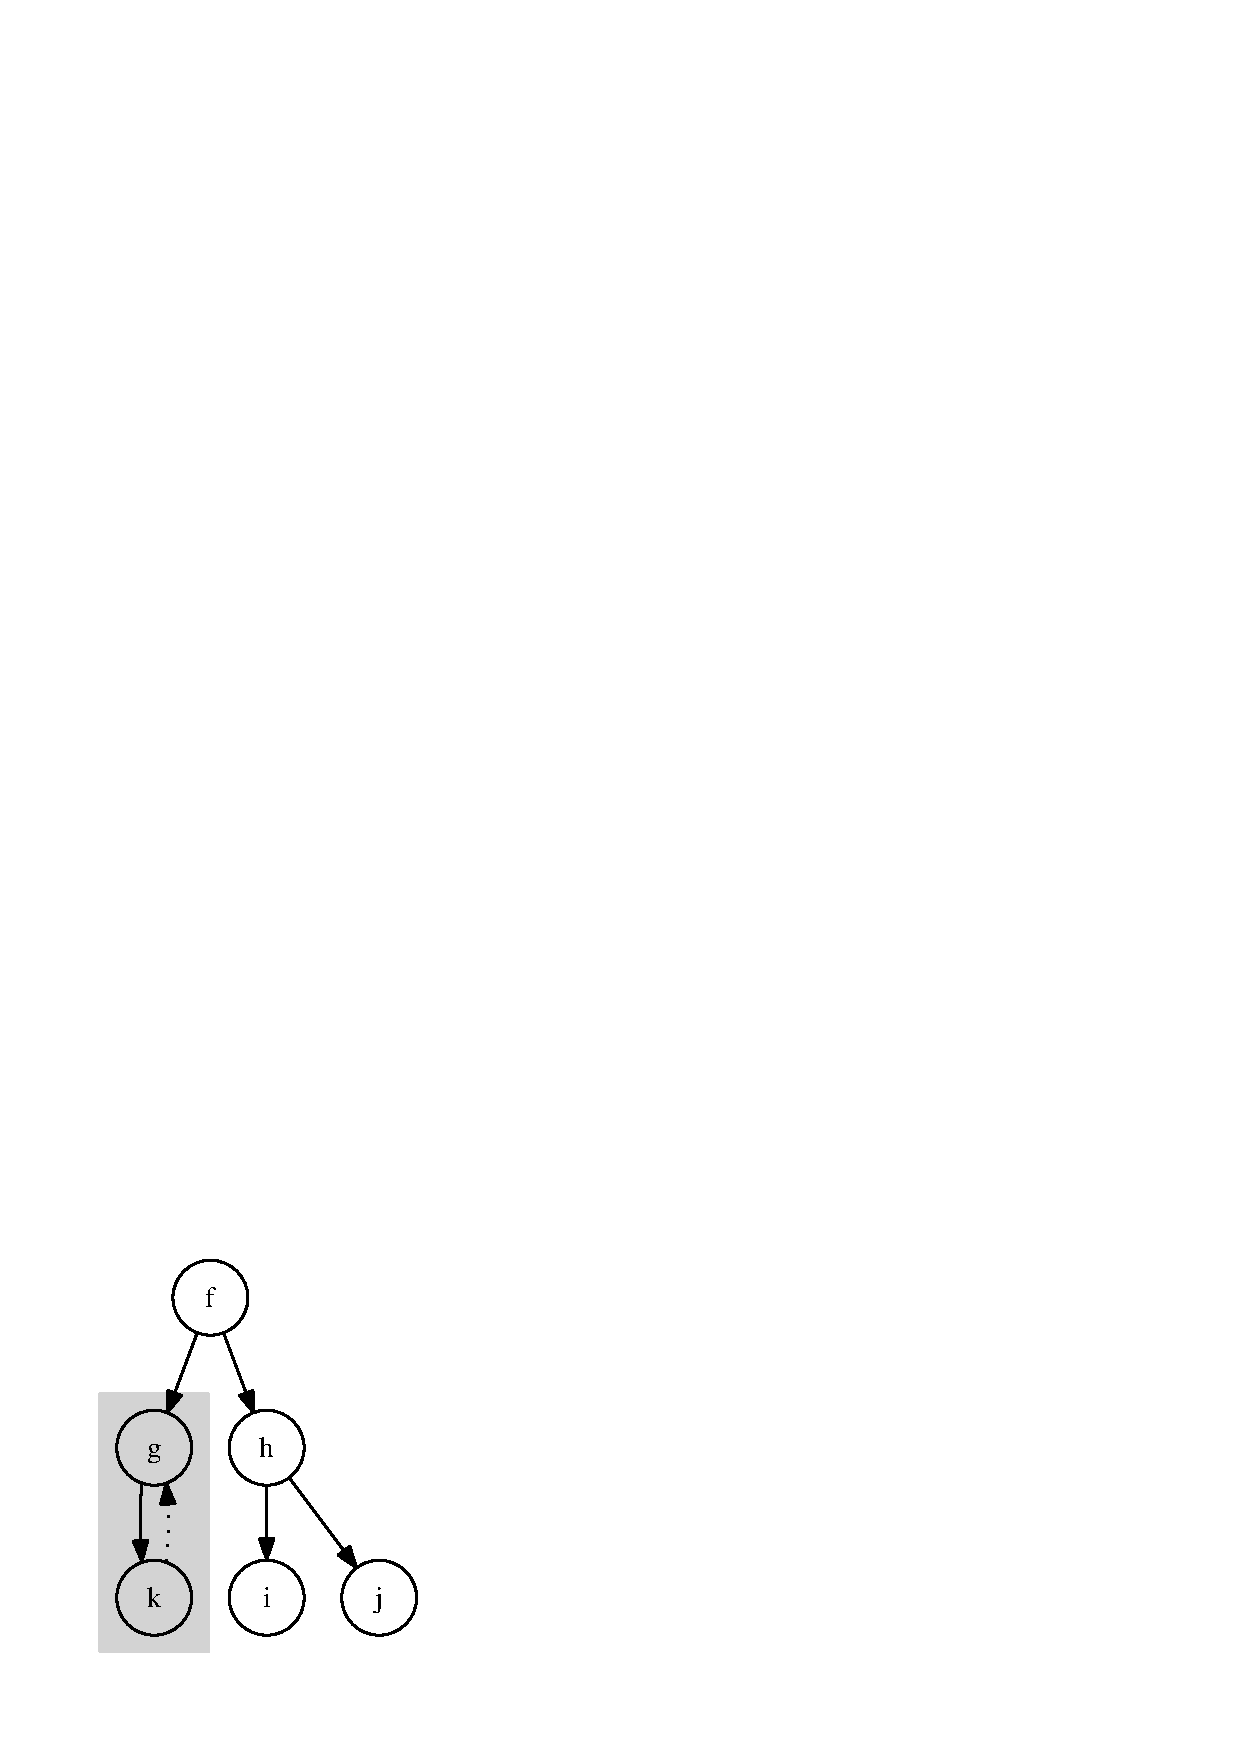
\includegraphics[scale=0.75]{call_graph} %\cline{1-1}
     &
      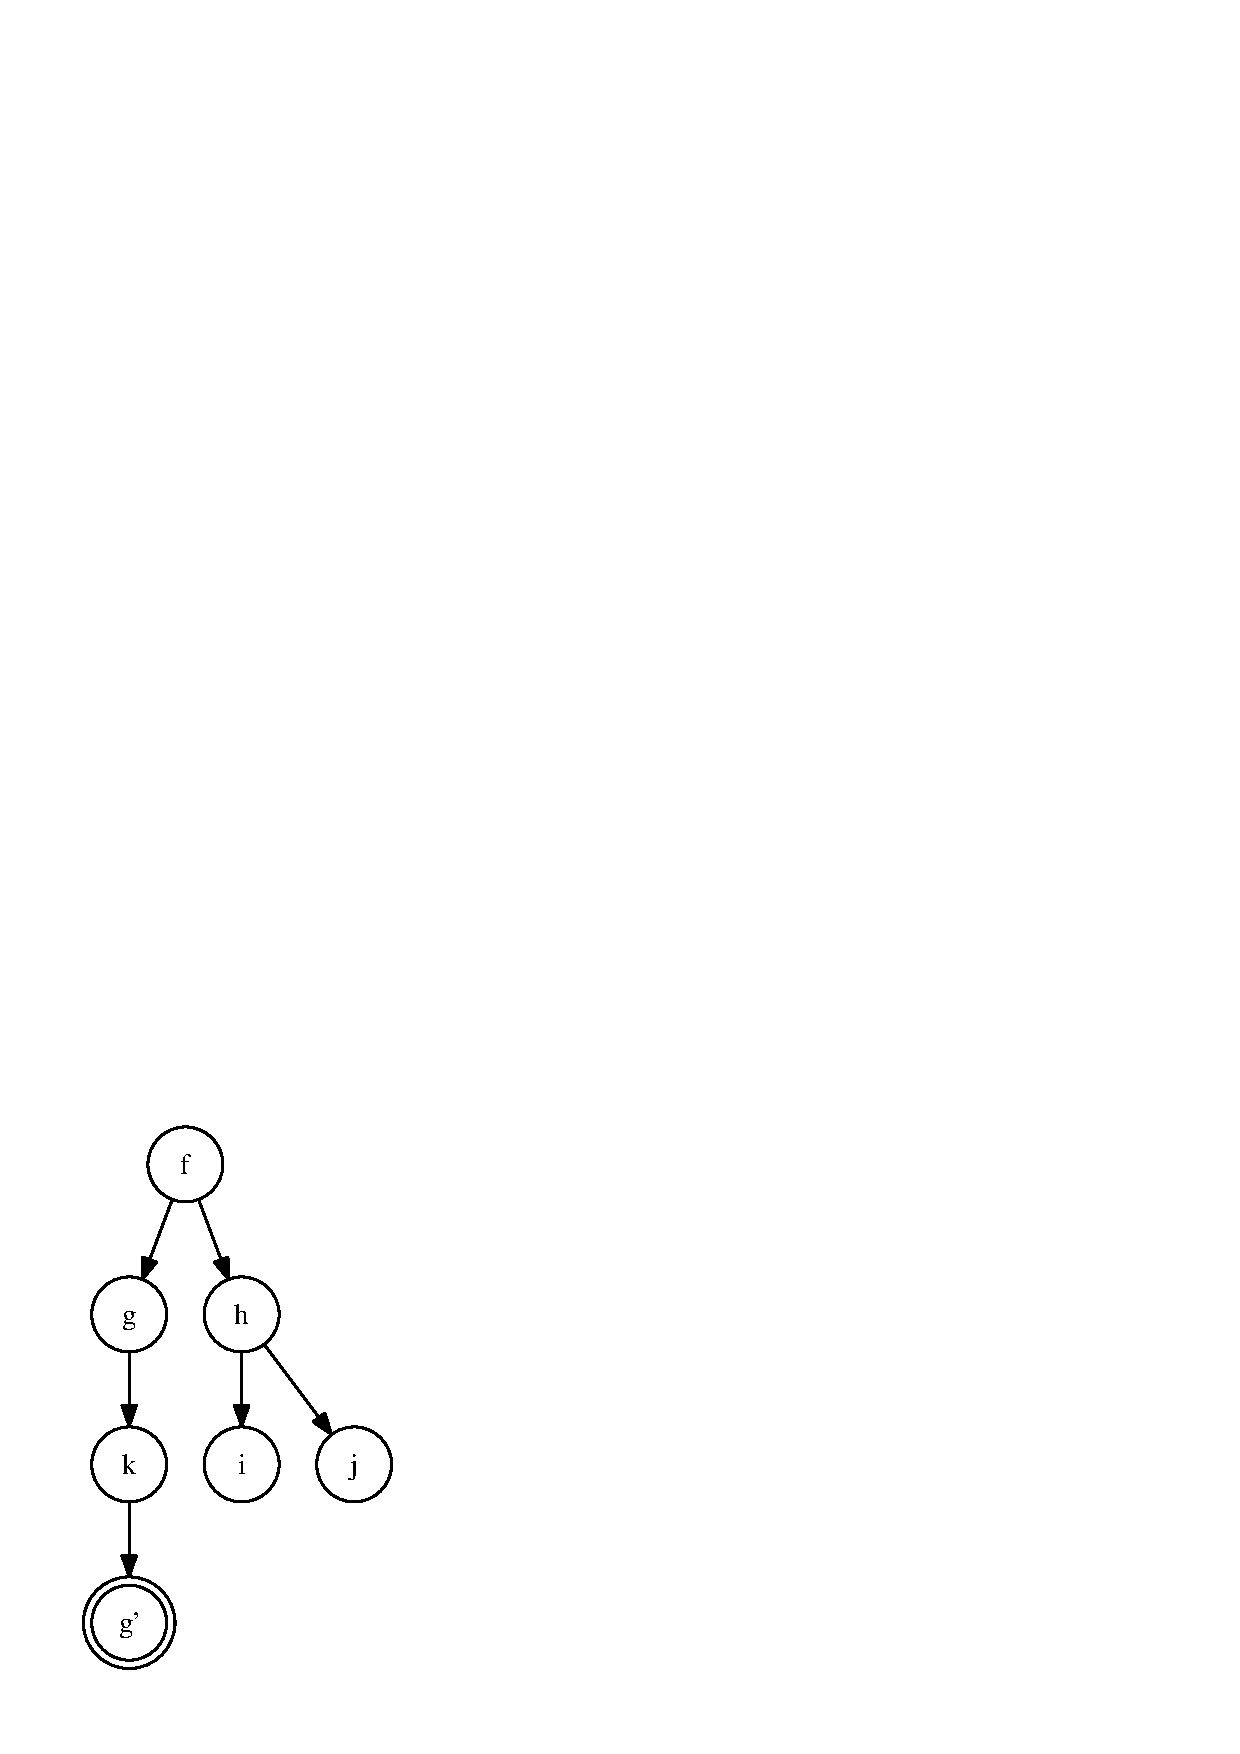
\includegraphics[scale=0.75]{ordered_graph} \\
     (a) Cyclic call graph & 
     (b) Corresponding DAG \\
    \end{tabular}}
  \end{center}
\end{figure}
}
\subsection{Computing Abstract Summary}
\frame
{
	\begin{figure}
  \begin{center}
    \scalebox{.65}{\begin{tabular}{| c | c | }
    \hline
    \multirow{2}{*}{{\tt
\begin{program}{0}
%  \FL\ \ldots
  \NL{0} procedure f(p) 
  \NL{0} begin
  \NL{1}  q = p\rtarrow{next};
  \NL{1}  g(q);
  \NL{0}  end
  \NL{0} procedure g(r)
  \NL{0}  begin
  \NL{1}  $\cdots$ = r\rtarrow{num};
  \NL{1}  s = r\rtarrow{next};
  \NL{1}  s\rtarrow{num}=$\cdots$;
  \NL{0}  end
 \end{program}
 
}} %\cline{1-1}
     & \\
    & 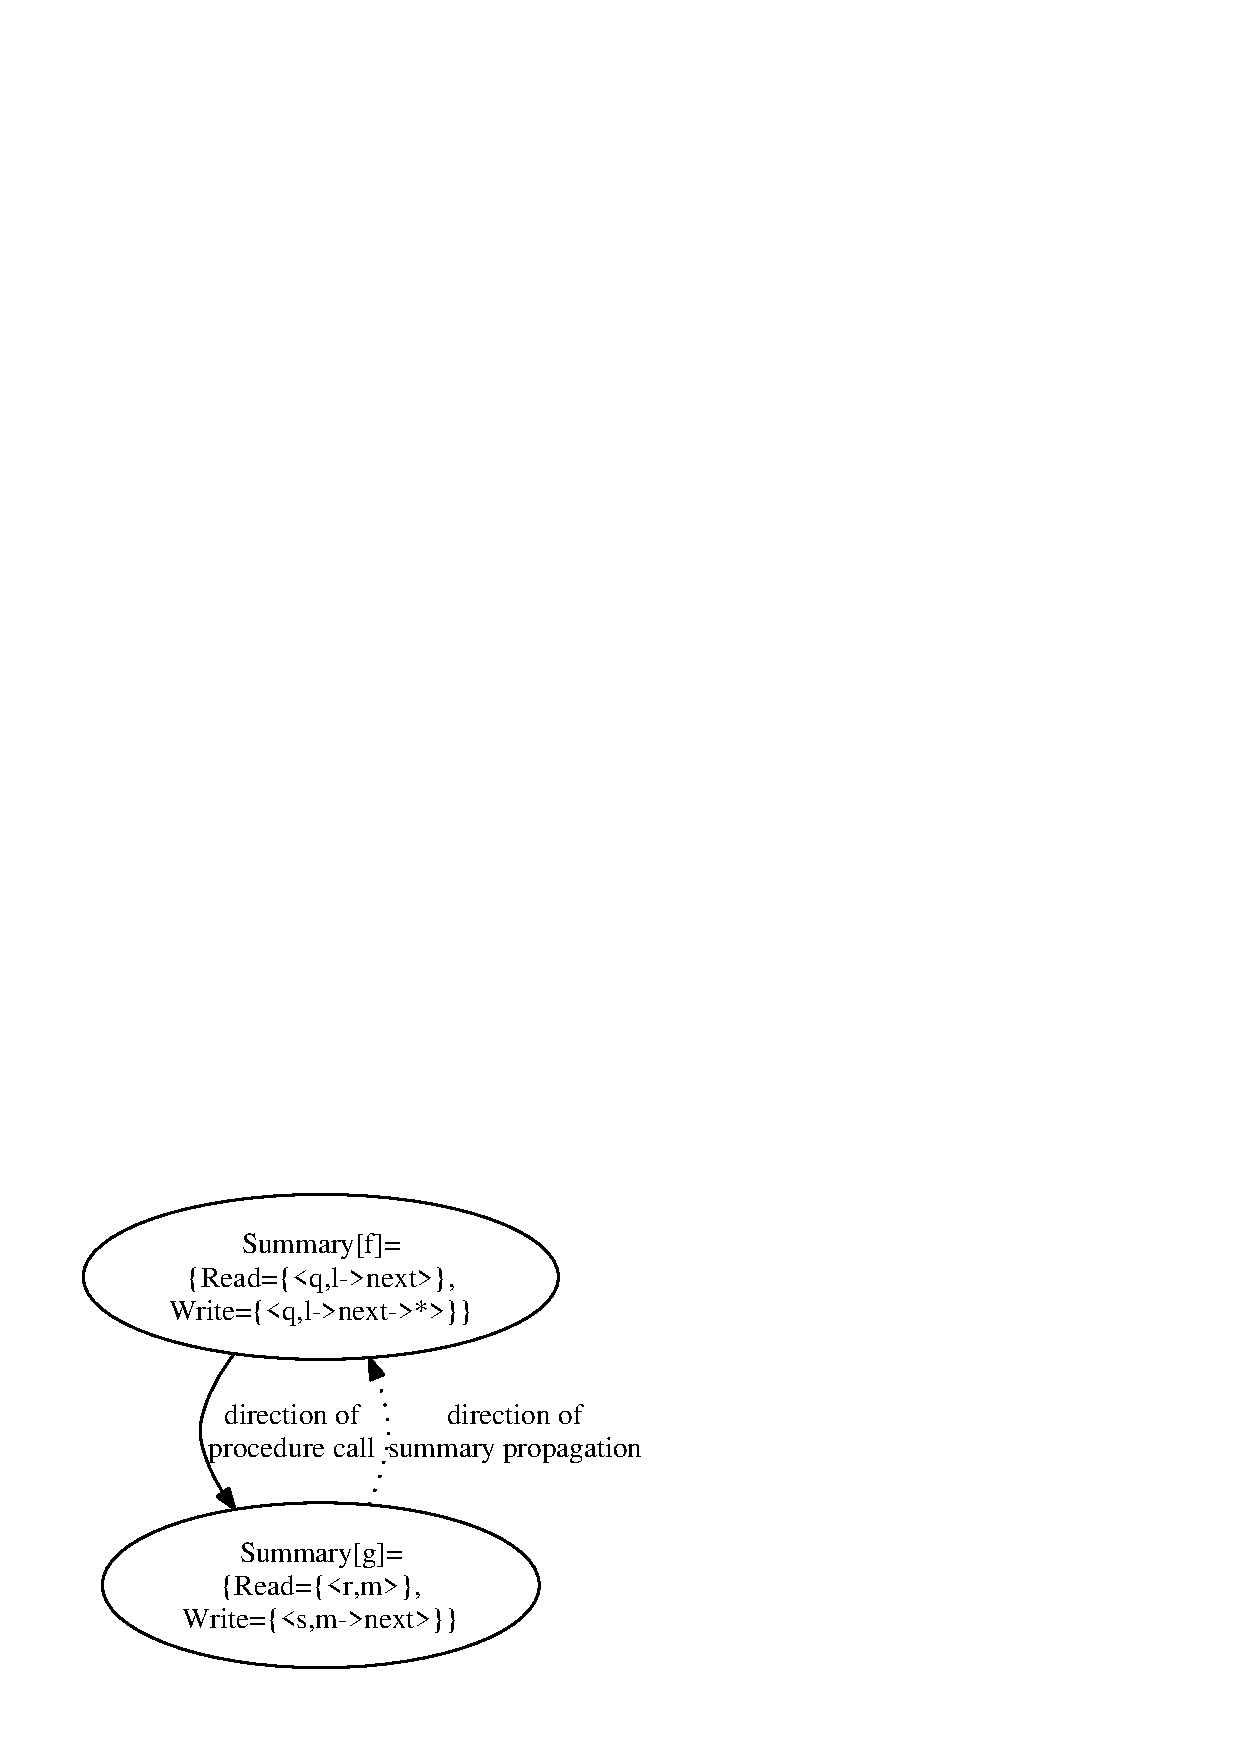
\includegraphics[scale=0.6]{grph5} \\
%      & \\
 %     & \\
%      \includegraphics[scale=0.6]{grph_RD_WR} & \\
%     (a) & (b) \\
	& \\
      (a) Example program with procedure call &
     (b) Call graph showing summary of procedures \\
     \hline
%     \hline
    \end{tabular}}
  \end{center}
%  \hrule
%  \caption{\label{fig:codeInter} Example showing computation of abstract summary}
%\hrule
\end{figure}
}
\section{Related Work}
\subsection{Related Work}
\frame
{
	\frametitle{\subsecname}
	\begin{itemize}
	\item Work done by Ghiya et. al\footnote{Rakesh Ghiya, Laurie Hendren and Yingchun Zhu. Detecting parallelism in C programs with recursive data structures. \emph{Compiler Construction}, volume 1383 of \emph{Lecture Notes in Computer Science}, pages 159-173. }
	\begin{itemize}
	\item uses coarse shape attribute of data structure
	\item computes complete access paths in terms of anchor pointer
	\item tests for aliases of access paths using shape information
	\item imprecise and conservative
	\end{itemize}
	\end{itemize}
}
\frame
{
	\frametitle{\subsecname}
	\begin{itemize}
	\item Work done by Navarro et. al\footnote{A. Navarro, F. Corbera, R. Asenjo, A. Tineo, O. Plata and E. Zapata. A New Dependence Test Based on Shape Analysis for Pointer-Based Codes. In \emph{the 17th International Workshop on Languages and Compilers for Parallel Computing}, September 2004.}
	\begin{itemize}
	\item obtains Reference Shape Graph of heap structure
	\item tags nodes with read and write access
	\item identifies dependences based on tagging information
	\item expensive in time
	\end{itemize}
	\end{itemize}
		
}

\section{Future Work}
%\subsection{Future Work}
\frame
{
	\frametitle{\secname}
	\begin{itemize}
	\item Improving of summarization technique
	\end{itemize}
	\pause
	\begin{itemize}
	\item Developing shape analysis technique to handle complex and cyclic structures
	\end{itemize}
	\pause
	\begin{itemize}
	\item Extending loop sensitive analysis to handle irregular control flow constructs
	\end{itemize}	
	\pause
	\begin{itemize}
	\item Further developing prototype model to handle large benchmarks
	\end{itemize}
	\pause
	\begin{itemize}
	\item Extending prototype model to implement interprocedural analysis
	\end{itemize}
	
}

\begin{frame}[plain]

	\begin{center}
	\Huge{\emph{\blue Thank You !!!}}
	\end{center}

\end{frame}

%\nocite{*}
%\bibliographystyle{alpha}
%\bibliography{reference}
\end{document}

